\documentclass[11pt]{scrartcl}
\usepackage[sexy]{evan}
\usepackage{graphicx}
\graphicspath{ {./images/} }

\usepackage{answers}
\Newassociation{hint}{hintitem}{all-hints}
\renewcommand{\solutionextension}{out}
\renewenvironment{hintitem}[1]{\item[\bfseries #1.]}{}

\usepackage{venndiagram,multicol,hyperref,graphicx,array}

\begin{document}
\title{Juegos}
\author{Ricardo Largaespada}
\date{06 Abril 2024}

\maketitle

\section{Introducción}

Cuando hablamos de juegos, pensamos en varios conocidos como: ajedrez, las damas y los juegos con baraja. Sin embargo, no son de estos juegos de los que vamos a hablar en este material. ¡Imagina que exista algún tipo de juego en el que pudieras ganar siempre, independientemente de cómo juegue tu adversario! ¡Sería bueno, ¿verdad?! Pues estos juegos existen y son uno de los temas más tratados en las pruebas de olimpiadas. En esta clase vamos a mostrar varios de estos juegos y las principales estrategias ganadoras: la simetría y el uso de las posiciones ganadoras.


\section{Simetría}
Una de las estrategias más simples es el uso de alguna simetría que pueda ocurrir durante el juego en ventaja de uno de los jugadores, forzando siempre una nueva ronda para el jugador ``destinado a la derrota''. Para entender mejor, vea el siguiente ejemplo.

\begin{example}
Pedro y Mónica juegan en un tablero de 1 $\times$ 11. Cada uno, a su turno, puede pintar uno de los cuadrados (que no hayan sido pintados previamente) o dos cuadrados consecutivos (si ambos están blancos). Quien no pueda jugar más pierde. Se sabe que Pedro será el primero en jugar. ¿Quién puede garantizar siempre la victoria?
\end{example}
Pedro siempre podrá ganar si sigue la siguiente estrategia:
\begin{enumerate}
    \item Inicialmente, Pedro debe pintar el cuadrado del medio.
    \begin{center}
        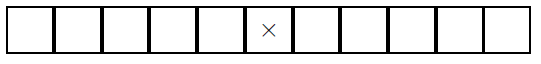
\includegraphics[scale=1]{images/clase_06_eje1.png}
    \end{center}
    \item Ahora, después de que Mónica haga su jugada, Pedro debe jugar siempre simétricamente con respecto al centro del tablero (es decir, manteniendo el tablero simétrico). Por ejemplo, si Mónica juega en las casillas 9 y 10, Pedro debe jugar en las casillas 2 y 3.
    \begin{center}
        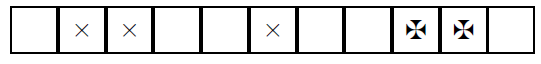
\includegraphics[scale=1]{images/clase_06_eje1-2.png}
    \end{center}
    \item De esta manera, Mónica nunca podrá ganar, ya que en su jugada ella "rompe la simetría" y la configuración final del juego tendrá todas las casillas pintadas, es decir, la configuración es simétrica.
\end{enumerate}

El próximo ejemplo es uno de los problemas que apareció en la prueba de la Olimpiada Brasileira de Matemática (OBM) de 2004. Vamos a presentar una solución diferente a la solución propuesta en Eureka! 22, usando simetría.

\begin{example}
Arnaldo y Bernardo disputan un juego en un tablero $2 \times n$. Las piezas del juego son dominós de $2 \times 1$.
\begin{center}
    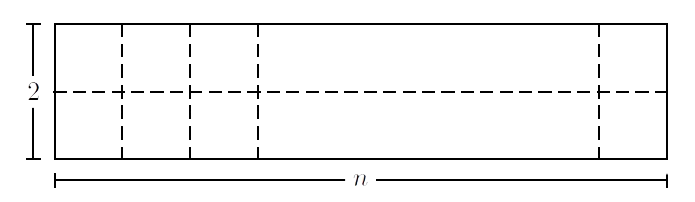
\includegraphics[scale=0.4]{images/clase_06_eje2.png}
\end{center}
Inicialmente, Arnaldo coloca un dominó cubriendo exactamente dos casillas del tablero, ya sea en horizontal o en vertical. Los jugadores se turnan para colocar una pieza en el tablero, ya sea en horizontal o en vertical, siempre cubriendo exactamente dos casillas del tablero. No se permite colocar una pieza sobre otra que ya haya sido colocada anteriormente. Quien no pueda colocar una pieza en el tablero pierde.

¿Cuál de los dos jugadores tiene una estrategia ganadora, es decir, una estrategia que lo lleva a la victoria sin importar las jugadas de su oponente, para:
\begin{enumerate}[a)]
    \item $n = 2004$?
    \item $n = 2005$?
\end{enumerate}
\end{example}
Cuando \( n = 2005 \), el primer jugador garantiza la victoria. Puede lograrlo colocando un dominó en posición vertical en el medio del tablero y luego jugando simétricamente al segundo jugador. Cuando \( n = 2004 \), el tablero tiene un número par de columnas. Por lo tanto, el segundo jugador gana jugando simétricamente al primer jugador.\\

Como habrás visto, utilizar la simetría es realmente una técnica muy eficaz. Sin embargo, a veces, utilizar únicamente la simetría no es suficiente para resolver el problema. Observa el siguiente ejemplo tomado de la Olimpiada de Bielorrusia de 2000.

\begin{example}
Tom y Jerry juegan el siguiente juego. Alternativamente, colocan alfileres idénticos en casillas vacías de un tablero de 20 $\times$ 20 (un alfiler a la vez). Tom es el primero en jugar. Gana quien, en su jugada, forme un bloque de cuatro alfileres adyacentes. Dos alfileres son adyacentes si están en casillas con un lado en común. Determina quién tiene la estrategia ganadora.
\end{example}
Jerry debe jugar simétricamente con respecto al centro del tablero. Tan pronto como Tom forme un bloque de tres alfileres adyacentes, Jerry debe abandonar la estrategia simétrica y completar el bloque de cuatro alfileres adyacentes.

\section{Posiciones Vencedoras}

Algunos tipos de juegos tienen ciertas configuraciones que siempre conducen a la victoria de un jugador. Estas configuraciones se llaman posiciones ganadoras. El siguiente ejemplo es un juego bastante simple en el que esta estrategia aparece fácilmente.

\begin{example}
En la primera casilla de un tablero de $1 \times 13$ hay una moneda. Tiago y María mueven la moneda alternadamente. En cada turno se permite avanzar 1, 2, 3, 4 o 5 casillas. Quien coloque la moneda en la última casilla es el ganador. Si María comienza a jugar, ¿puede estar segura de la victoria?
\end{example}
Como en muchos problemas de olimpiada, vamos a analizar algunos casos pequeños. Supongamos que en lugar de tener 13 casillas, el tablero tuviera solo cuatro. En este caso, es fácil ver que quien comienza gana, basta con avanzar tres casillas. \\
Lo mismo ocurriría si el tablero tuviera 2, 3, 4, 5 o 6 casillas. Sin embargo, en un tablero $7 \times 1$ el primer jugador pierde. Observa que después del primer movimiento, la moneda estará en una de las casillas 2, 3, 4, 5 o 6. Y ya sabemos que estas casillas llevan al jugador a la victoria. \\
\begin{center}
    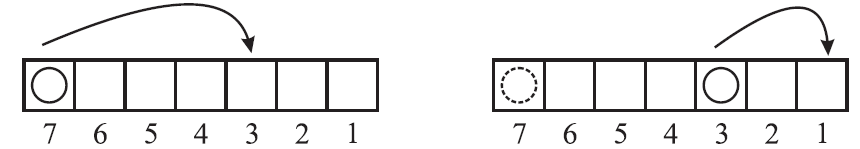
\includegraphics[scale=0.8]{images/clase_06_eje3.png}
\end{center}
Por lo tanto, diremos que 7 es una posición perdedora y 6, 5, 4, 3 y 2 son posiciones ganadoras. Así, si un jugador está en una de las casillas 8, 9, 10, 11 o 12, puede garantizar la victoria moviendo la moneda a la casilla 7, dejando a su oponente en una posición perdedora. Con esto, podemos afirmar que las posiciones 8, 9, 10, 11 y 12 también son posiciones ganadoras. \\
Solo queda analizar la casilla 13. Observa que desde esta casilla solo podemos mover la moneda a una de las casillas 8, 9, 10, 11 o 12, que son ganadoras. Por lo tanto, quien comience pierde debido al simple hecho de comenzar en una posición perdedora.\\

La gran dificultad para la mayoría de los alumnos es descubrir cuáles son las posiciones ganadoras de un juego. Para evitar este tipo de problema, siempre ten en mente las siguientes definiciones:
\begin{definition}[Posición ganadora] A partir de ella, podemos elegir un movimiento y pasar una posición perdedora al adversario.
\end{definition}
\begin{definition}[Posición perdedora] A partir de ella, es imposible elegir un movimiento y pasar una posición perdedora al adversario. Es decir, no importa el movimiento elegido, el adversario recibirá una posición ganadora.
\end{definition}

Para descubrir cuáles son las posiciones ganadoras y perdedoras, la mejor manera es analizar el final del juego y aplicar las definiciones proporcionadas anteriormente. Vamos a practicar un poco resolviendo el próximo problema.

\begin{example}
En un tablero de ajedrez de $8 \times 8$, una torre está en la casilla a1. Dos jugadores mueven la torre con el objetivo de colocarla en la casilla h8. Sabiendo que la torre solo puede moverse hacia arriba o hacia la derecha (tantas casillas como el jugador desee) y que no se puede perder el turno, determina qué jugador tiene la estrategia ganadora.
\end{example}
Primero, note que todas las casillas de la última fila y de la última columna (excepto h8) son ganadoras, ya que desde ellas podemos elegir un movimiento que nos lleve a la victoria. Con eso, la casilla g7 se convierte en perdedora, ya que desde ella cualquier movimiento lleva al otro jugador a una posición ganadora (ver figura 1).
\begin{center}
    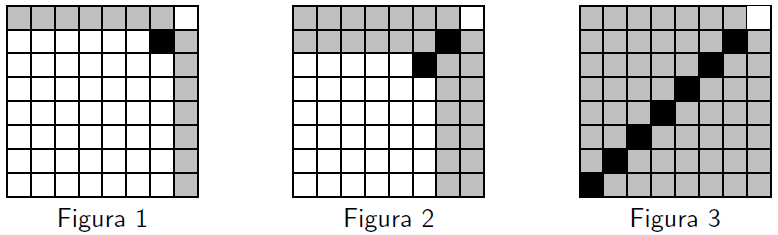
\includegraphics[scale=0.8]{images/clase_06_eje4.png}
\end{center}
Ahora, como g7 es perdedora, las demás casillas de la séptima fila y de la séptima columna son ganadoras. Además, la casilla f6 también debe ser perdedora (ver figura 2). Continuando de manera análoga, obtenemos que la casilla a1 es perdedora (ver figura 3). Por lo tanto, quien comience, pierde.
\Opensolutionfile{all-hints}

\section{Problemas Propuestos}
\begin{problem}
Sobre una mesa hay dos pilas (una con 15 y otra con 16 piedras). En un juego, cada jugador puede, en su turno, retirar cualquier cantidad de piedras de solo una pila. Quien no pueda jugar más, pierde. ¿Quién tiene la estrategia ganadora?
\begin{hint}
El jugador 1 debe retirar una piedra de la pila con 16. Luego, debe jugar simétricamente con respecto al jugador 2.
\end{hint}
\end{problem}

\begin{problem}
Dos jugadores colocan alternativamente alfiles (del mismo color) en un tablero de $8 \times 8$, de manera que ningún alfil ataque a otro. Quien no pueda jugar más, pierde.
\begin{hint}
    Divida el tablero en dos partes, cada una formada por 4 filas. El jugador 1 debe jugar simétricamente luego.
\end{hint}
\end{problem}

\begin{problem}
Dos jugadores colocan alternativamente reyes (del mismo color) en un tablero de $9 \times 9$, de manera que ningún rey ataque a otro. Quien no pueda jugar más, pierde.
\begin{hint}
    El primer jugador debe colocar un rey en el centro y luego jugar simétricamente con respecto al centro del tablero.
\end{hint}
\end{problem}

\begin{problem}
Se da un tablero de ajedrez ($8 \times 8$) y palitos del tamaño de los lados de las casillas del tablero. Dos jugadores juegan alternativamente y, en cada turno, uno de los jugadores coloca un palito sobre un lado de una de las casillas del tablero, estando prohibido superponer los palitos. Gana el jugador que logre completar primero un cuadrado de $1 \times 1$ con palitos. Suponiendo que ninguno de los jugadores cometa errores, ¿cuál de los dos tiene la estrategia ganadora?
\end{problem}

\begin{problem}
Se dan veinte puntos alrededor de un círculo. Cada jugador, en su turno, puede unir dos de estos puntos si el nuevo segmento no corta los segmentos previamente trazados. Quien no pueda trazar ningún segmento más, pierde.
\end{problem}

\begin{problem}
Dos jugadores colocan alternativamente X's y O's en un tablero de $9 \times 9$. El primero coloca X's y el segundo O's. Cuando el tablero esté completamente lleno, el juego termina y se cuentan los puntos. Se da un punto al jugador por cada fila o columna en la que tenga más casillas que el adversario. El jugador que tenga más puntos, gana. ¿Quién puede ganar siempre?
\end{problem}

\begin{problem}
Un peón está en el centro de un tablero de $11 \times 11$. Dos jugadores mueven alternativamente al peón a cualquier otra casilla del tablero, pero en cada movimiento (a partir del segundo), la casilla elegida debe ser mayor que la anterior. El jugador que no pueda jugar más, pierde. Encuentra la estrategia ganadora.
\end{problem}

\begin{problem}Un juego consiste en romper un tablero de $5 \times 10$ a lo largo de sus líneas. Gana el primer jugador que obtenga un cuadrado de $1 \times 1$. ¿Quién tiene la estrategia ganadora?
\end{problem}

\begin{problem}[Rusia 1997] Los números 1, 2, 3, ..., 1000 se escriben en la pizarra. Dos jugadores borran alternativamente uno de los números de la lista hasta que queden solo dos números. Si la suma de estos números es divisible por 3, gana el primer jugador; de lo contrario, gana el segundo. ¿Quién tiene la estrategia ganadora?
\begin{hint}
    Observa que la suma de dos elementos opuestos siempre es 1002, que es un múltiplo de 3.
\end{hint}
\end{problem}

\begin{problem}
En una mesa hay dos pilas de monedas, cada una con 11 monedas. En cada turno, un jugador puede retirar dos monedas de una de las pilas o una moneda de cada pila. El jugador que no pueda realizar más movimientos, pierde.
\begin{hint}
    Construye un tablero de 11x11, donde la casilla (i, j) represente la cantidad de piedras en cada pila. Observa que el movimiento del juego original es equivalente al movimiento del caballo en el tablero. Termina el problema descubriendo las posiciones ganadoras y perdedoras a través de la inducción retroactiva.
\end{hint}
\end{problem}

\begin{problem}
Tom y Jerry juegan un juego y Tom da el primer paso. En cada turno, el jugador puede reducir en un número natural N uno de sus dígitos no nulos. Inicialmente, el número N es 1234. El jugador que obtenga cero, gana. ¿Quién puede garantizar la victoria?
\end{problem}

\begin{problem}
Se da una pila de 500 piedras. Dos jugadores juegan el siguiente juego: en cada turno, el jugador puede retirar 1, 2, 4, 8,... (cualquier potencia de 2) piedras de la pila. El jugador que no pueda jugar más, pierde.
\begin{hint}
    Piensa en los múltiplos de 3. Ninguna potencia de 2 es múltiplo de 3.
\end{hint}
\end{problem}

\begin{problem}
    En una caja hay 300 bolitas. Cada jugador puede retirar no más de la mitad de las bolitas que están en la caja. El jugador que no pueda jugar más, pierde.
\begin{hint}
     Piensa en las potencias de 2.
\end{hint}
\end{problem}
\begin{problem}
En una mesa hay dos pilas (una con 7 y otra con 15 piedras). En un juego, cada jugador puede, en su turno, retirar cualquier cantidad de piedras de solo una pila o la misma cantidad de ambas pilas. El jugador que no pueda jugar más, pierde. ¿Quién tiene la estrategia ganadora?
\begin{hint}
Nuevamente, usa la idea del tablero que se usó para resolver el problema 15.
\end{hint}
\end{problem}

\Closesolutionfile{all-hints}

\section{Sugerencias y Soluciones}
\begin{enumerate}
\input{all-hints.out}
\end{enumerate}

\end{document}